\documentclass[12pt]{article}

\usepackage[a4paper, margin=1in]{geometry}
\usepackage{array}
\usepackage{multirow}
\usepackage{setspace}
\usepackage{tikz}
\usepackage{pgfplots}
\usepackage{tfrupee}
\usepackage{amssymb ,amsmath ,amsfonts}
\usetikzlibrary{shapes,positioning ,arrows.meta}
\usepackage[utf8]{inputenc}
\usetikzlibrary{calc}

\begin{document}

\begin{center}
    \textbf{\Large  Data Science and Artificial Intelligence - DA}
\end{center}

\noindent \textbf{\underline{General Aptitude}}
\vspace{0.2cm}

\noindent
\textbf{Q.1 - Q.5 Carry ONE mark Each}

\vspace{0.5cm}

\renewcommand{\arraystretch}{1.8}

\begin{tabular}{|p{1.5cm}|p{12cm}|}
\hline

\textbf{Q.1} &
Courage : Bravery :: Yearning : \rule{3cm}{0.4pt}

\vspace{0.3cm}

Select the most appropriate option to complete the analogy.
\\
\hline

(A) & Longing \\
\hline

(B) & Yelling \\
\hline

(C) & Yawning \\
\hline

(D) & Glaring \\
\hline

\end{tabular}


\vspace{0.5cm}

\renewcommand{\arraystretch}{1.8}

\begin{tabular}{|p{1.5cm}|p{12cm}|}
\hline

\textbf{Q.2} &

We \rule{2cm}{0.4pt} tennis in the lawn when it suddenly started to rain. 

\vspace{0.3cm}

Select the most appropriate option to complete the above sentence..
\\
\hline

(A) & have been playing \\
\hline

(B) & had been playing \\
\hline

(C) & would have been playing \\
\hline

(D) & could be playing \\
\hline

\end{tabular}



\vspace{0.5cm}

\renewcommand{\arraystretch}{1.8}

\begin{tabular}{|p{1.2cm}|p{12cm}|}
\hline
\textbf{Q.3} &
A $4 \times 4$ digital image has pixel intensities ($U$) as shown in the figure. 
The number of pixels with $U \leq 4$ is:
\\
\hline

& 
\vspace{0.000001cm}
\begin{center}
\begin{tabular}{|c|c|c|c|}
\hline
0 & 1 & 0 & 2 \\ \hline
4 & 7 & 3 & 3 \\ \hline
5 & 5 & 4 & 4 \\ \hline
6 & 7 & 3 & 2 \\ \hline
\end{tabular}
\end{center}
\vspace{0.01cm}
\\
\hline

(A) & 3 \\
\hline

(B) & 8 \\
\hline

(C) & 11 \\
\hline

(D) & 9 \\
\hline

\end{tabular}


\vspace{0.5cm}

\renewcommand{\arraystretch}{1.8}
\begin{tabular}{|p{1.2cm}|p{12cm}|}
\hline
\textbf{Q.4} &
In the given figure, the numbers associated with the rectangle, triangle, and ellipse 
are 1, 2, and 3, respectively. Which one among the given options is the most 
appropriate combination of P, Q, and R? \\
\hline

& 
\begin{center}
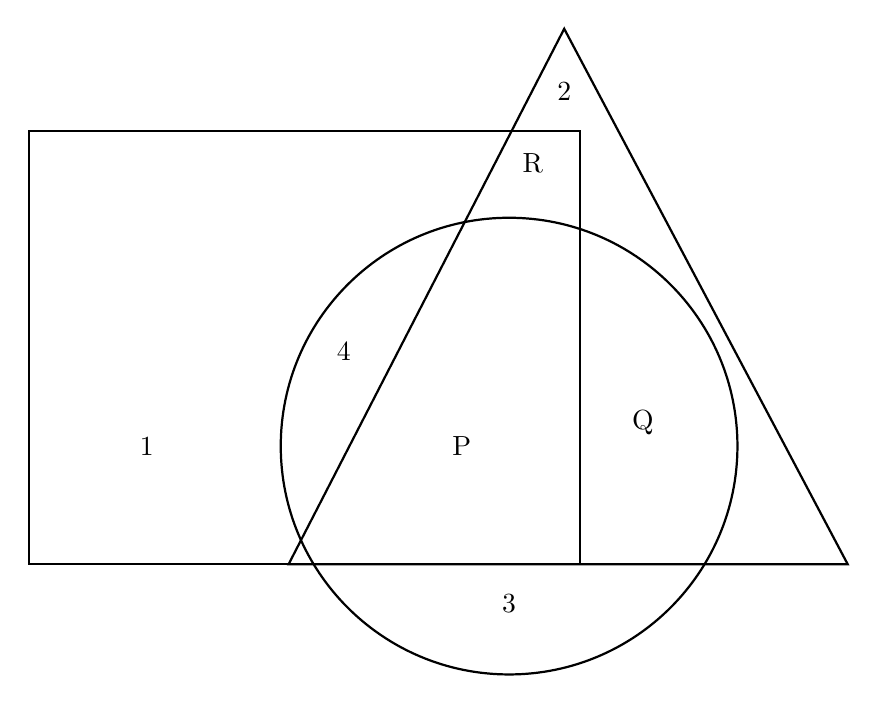
\begin{tikzpicture}[thick]
    
    \draw (0,0) rectangle (7,5.5);
    
    
    \draw (3.3,0) --  (6.8,6.8) -- (10.4,0) -- cycle;
    

    \draw (6.1,1.5) circle (2.9);
    

    \node at (1.5,1.5) {1};
    
    
    \node at (6.8,6) {2};
    
    
    \node at (6.1,-0.5) {3};
    

    \node at (4,2.7) {4};
    
    
    \node at (5.5,1.5) {P};
    
    
    \node at (7.8,1.8) {Q};
    
    
    \node at (6.4,5.1) {R};

\end{tikzpicture}
\end{center}
\\
\hline

(A) & $P = 6; \ Q = 5; \ R = 3$ \\
\hline

(B) & $P = 5; \ Q = 6; \ R = 3$ \\
\hline

(C) & $P = 3; \ Q = 6; \ R = 6$ \\
\hline

(D) & $P = 5; \ Q = 3; \ R = 6$ \\
\hline

\end{tabular}

\vspace{0.5cm}

\renewcommand{\arraystretch}{1.8}
\begin{tabular}{|p{1.2cm}|p{12cm}|}
\hline
\textbf{Q.5} &

\noindent A rectangle has a length $L$ and a width $W$, where $L > W$. If the width, $W$, is increased by 10\%, which one of the following statements is correct for all values of $L$ and $W$?
\\
\hline

(A) & Perimeter increases by 10\%.  \\
\hline

(B) & Length of the diagonals increases by 10\%. \\
\hline

(C) & Area increases by 10\%.\\
\hline

(D) & The rectangle becomes a square. \\
\hline

\end{tabular}

\vspace{3.5cm}

\noindent \textbf{Q.6 - Q.10 Carry TWO marks Each}

\vspace{0.5cm}

\renewcommand{\arraystretch}{1.8}
\begin{tabular}{|p{1.2cm}|p{12cm}|}
\hline
\textbf{Q.6} & 
Column-I has statements made by Shanthala; and, Column-II has responses given by Kanishk.

\begin{center}
\renewcommand{\arraystretch}{1.5}
\begin{tabular}{|c|p{4.5cm}|c|p{4.5cm}|}
\hline
\multicolumn{2}{|c|}{Column-I} & \multicolumn{2}{c|}{Column-II} \\ \hline
P. & This house is in a mess. & 1. & Alright, I won't bring it up during our conversations. \\ \hline
Q. & I am not happy with the marks given to me. & 2. & Well, you can easily look it up. \\ \hline
R. & Politics is a subject I avoid talking about. & 3. & No problem, let me clear it up for you. \\ \hline
S. & I don't know what this word means. & 4. & Don't worry, I will take it up with your teacher. \\ \hline
\end{tabular}
\end{center}

Identify the option that has the correct match between Column-I and Column-II. \\ \hline

(A) & P -- 2; Q -- 3; R -- 1; S -- 4 \\ \hline
(B) & P -- 3; Q -- 4; R -- 1; S -- 2 \\ \hline
(C) & P -- 4; Q -- 1; R -- 2; S -- 3 \\ \hline
(D) & P -- 1; Q -- 2; R -- 4; S -- 3 \\ \hline
\end{tabular}
\vspace{0.5cm}

\renewcommand{\arraystretch}{1.8}
\begin{tabular}{|p{1.2cm}|p{12cm}|}
\hline
\textbf{Q.7} & 
Weight of a person can be expressed as a function of their age. The function usually varies from person to person. Suppose this function is identical for two brothers, and it monotonically increases till the age of 50 years and then it monotonically decreases. Let $a_1$ and $a_2$ (in years) denote the ages of the brothers and $a_1 < a_2$.

\vspace{0.3cm}
Which one of the following statements is correct about their age on the day when they attain the same weight? \\ \hline

(A) & $a_1 < a_2 < 50$ \\ \hline
(B) & $a_1 < 50 < a_2$ \\ \hline
(C) & $50 < a_1 < a_2$ \\ \hline
(D) & Either $a_1 = 50$ or $a_2 = 50$ \\ \hline
\end{tabular}

\vspace{0.5cm}

\renewcommand{\arraystretch}{1.8}
\begin{tabular}{|p{1.2cm}|p{12cm}|}
\hline
\textbf{Q.8} & 
A regular dodecagon (12-sided regular polygon) is inscribed in a circle of radius $r$ cm as shown in the figure. The side of the dodecagon is $d$ cm. All the triangles (numbered 1 to 12) in the figure are used to form squares of side $r$ cm and each numbered triangle is used only once to form a square. 

\vspace{0.3cm}
The number of squares that can be formed and the number of triangles required to form each square, respectively, are:

\vspace{0.3cm}
Note: The figure shown is representative. \\ \hline

 & 
\begin{center}
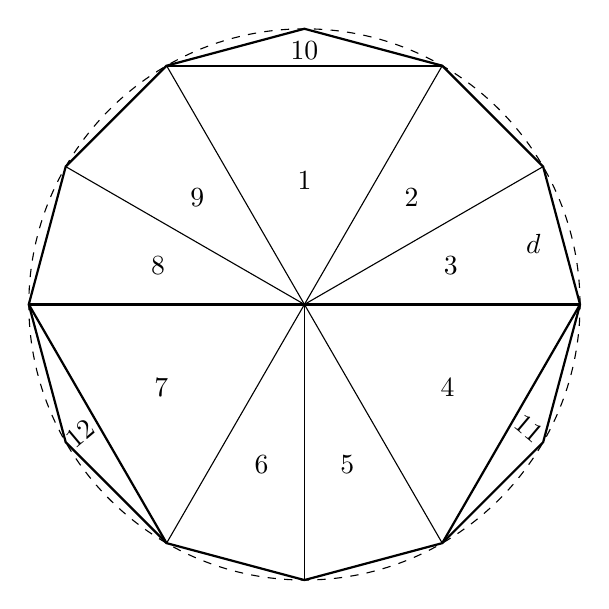
\begin{tikzpicture}[scale=3.5]
\def\r{1}


\foreach \i in {0,...,11}{
    \coordinate (P\i) at ({90-\i*30}:\r);
}


\draw[dashed, thin] (0,0) circle (\r);


\draw[thick] (P0) \foreach \i in {1,...,11}{ -- (P\i) } -- cycle;


\draw[thin] (0,0) -- (P1);
\draw[thin] (0,0) -- (P2);
\draw[thin] (0,0) -- (P3);

\draw[thin] (0,0) -- (P5);
\draw[thin] (0,0) -- (P6);
\draw[thin] (0,0) -- (P7);

\draw[thin] (0,0) -- (P9);
\draw[thin] (0,0) -- (P10);
\draw[thin] (0,0) -- (P11);


\draw[thick] (-1,0) -- (1,0);


\draw[thick] (P1) -- (P11);
\draw[thick] (P3) -- (P5);
\draw[thick] (P7) -- (P9);



\node at (90:0.45)  {1};   

\node at (45:0.55)  {2};
\node at (15:0.55)  {3};
\node at (-30:0.6)  {4};  

\node at (-75:0.6)  {5};
\node at (-105:0.6) {6};
\node at (-150:0.6) {7};   

\node at (165:0.55) {8};
\node at (135:0.55) {9};


\node at (90:0.92) {10};
\node[right] at (16:0.8) {$d$};
\node[rotate=-40] at (-29:0.93) {11}; 
\node[rotate=40] at (-150:0.94) {12};

\end{tikzpicture}
\end{center} \\ \hline

(A) & 3; 4 \\ \hline
(B) & 4; 3 \\ \hline
(C) & 3; 3 \\ \hline
(D) & 3; 2 \\ \hline
\end{tabular}
\vspace{0.5cm}

\renewcommand{\arraystretch}{1.8}
\begin{tabular}{|p{1.2cm}|p{12cm}|}
\hline
\textbf{Q.9} & 
If a real variable $x$ satisfies $3^{x^2} = 27 \times 9^x$, then the value of $\frac{2^{x^2}}{(2^x)^2}$ is: \\ \hline

(A) & $2^{-1}$ \\ \hline
(B) & $2^0$ \\ \hline
(C) & $2^3$ \\ \hline
(D) & $2^{15}$ \\ \hline
\end{tabular}
 
\pgfplotsset{compat=1.18}

\vspace{0.5cm}

\renewcommand{\arraystretch}{1.8}
\begin{tabular}{|p{1.2cm}|p{12cm}|}
\hline
\textbf{Q.10} & 
The number of patients per shift ($X$) consulting Dr. Gita in her past 100 shifts is shown in the figure. If the amount she earns
is \rupee $1000(X - 0.2)$, what is the average amount (in \rupee) she has earned per shift in the past 100 shifts?

\vspace{0.3cm}
Note: The figure shown is representative. \\ \hline

 & 
\begin{center}
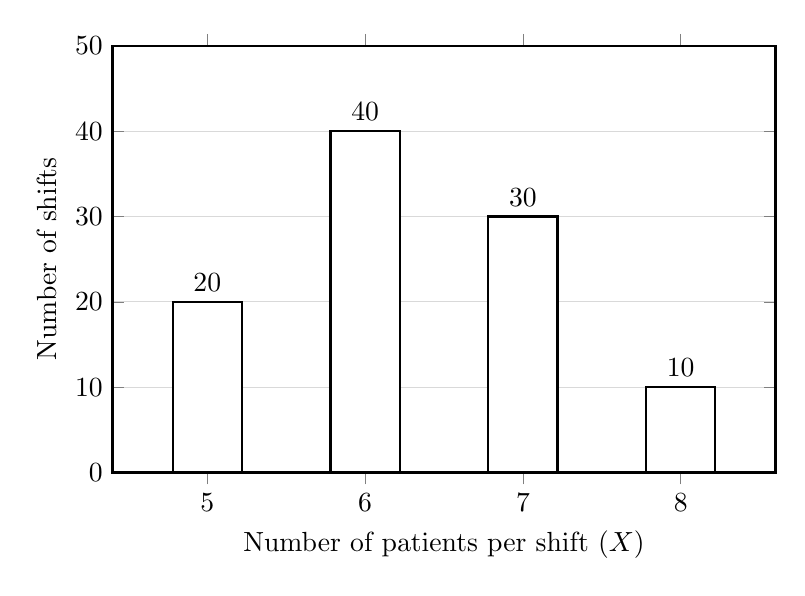
\begin{tikzpicture}
\begin{axis}[
    ybar,
    bar width=25pt,
    width=10cm,
    height=7cm,
    ymin=0, ymax=50,
    ytick={0,10,20,30,40,50},
    xtick={5,6,7,8},
    xlabel={Number of patients per shift ($X$)},
    ylabel={Number of shifts},
    nodes near coords,
    every node near coord/.append style={anchor=south},
    axis line style={thick},
    major grid style={draw=gray!30},
    ymajorgrids=true,
    enlarge x limits=0.2,
]
\addplot[fill=white, draw=black, thick] coordinates {(5,20) (6,40) (7,30) (8,10)};
\end{axis}
\end{tikzpicture}
\end{center} \\ \hline

(A) & 6,100 \\ \hline
(B) & 6,300 \\ \hline
(C) & 6,000 \\ \hline
(D) & 6,500 \\ \hline
\end{tabular}

\vspace{0.8cm}

\noindent \textbf{Q. 11 - Q. 35 carry one mark each.}

\vspace{0.5cm}

\noindent
\begin{tabular}{p{1cm} p{12.5cm}}
Q. 11 & Suppose $X$ and $Y$ are random variables. The conditional expectation of $X$ given $Y$ is denoted by $E[X|Y]$. Then $E[E[X|Y]]$ equals \\[5pt]
& (A) \quad $E[X|Y]$ \\[5pt]
& (B) \quad $\frac{E[X]}{E[Y]}$ \\[5pt]
& (C) \quad $E[X]$ \\[5pt]
& (D) \quad $E[Y]$ \\
\end{tabular}

\vspace{0.8cm}

\noindent
\begin{tabular}{p{1cm} p{12.5cm}}
Q. 12 & The number of additions and multiplications involved in performing Gaussian elimination on any $n \times n$ upper triangular matrix is of the order \\[5pt]
& (A) \quad $O(n)$ \\[5pt]
& (B) \quad $O(n^2)$ \\[5pt]
& (C) \quad $O(n^3)$ \\[5pt]
& (D) \quad $O(n^4)$ \\
\end{tabular}

\vspace{0.8cm}

\noindent
\begin{tabular}{p{1cm} p{12.5cm}}
Q. 13 & The sum of the elements in each row of $A \in \mathbb{R}^{n \times n}$ is 1.If $B = A^3 - 2A^2 + A$, which one of the following statements is correct (for $x \in \mathbb{R}^n$)? \\[5pt]
& (A) \quad The equation $Bx = 0$ has no solution \\[5pt]
& (B) \quad The equation $Bx = 0$ has exactly two solutions \\[5pt]
& (C) \quad The equation $Bx = 0$ has infinitely many solutions \\[5pt]
& (D) \quad The equation $Bx = 0$ has a unique solution \\
\end{tabular}

\vspace{0.8cm}

\noindent
\begin{tabular}{p{1cm} p{12.5cm}}
Q. 14 & Let $f(x) = \frac{e^x - e^{-x}}{2}, x \in \mathbb{R}$. Let $f^{(k)}(a)$ denote the $k^{th}$ derivative of $f$ evaluated at $a$. What is the value of $f^{(10)}(0)$? (Note: $!$ denotes factorial) \\[8pt]
& (A) \quad 0 \\[5pt]
& (B) \quad 1 \\[5pt]
& (C) \quad $\frac{1}{10!}$ \\[5pt]
& (D) \quad $\frac{2}{10!}$ \\
\end{tabular}

\vspace{0.8cm}

\noindent
\begin{tabular}{p{1cm} p{12.5cm}}
Q. 15 & Let $p$ and $q$ be any two propositions. Consider the following propositional statements. \\
& $S_1 : p \rightarrow q, \quad S_2 : \neg p \wedge q, \quad S_3 : \neg p \vee q, \quad S_4 : \neg p \vee \neg q,$ \\
& where $\wedge$ denotes conjunction (AND operation), $\vee$ denotes disjunction (OR operation), and $\neg$ denotes negation (NOT operation). Which one of the following options is correct? (Note: $\equiv$ denotes logical equivalence) \\[8pt]
& (A) \quad $S_1 \equiv S_3$ \\[5pt]
& (B) \quad $S_2 \equiv S_3$ \\[5pt]
& (C) \quad $S_2 \equiv S_4$ \\[5pt]
& (D) \quad $S_1 \equiv S_4$ \\
\end{tabular}

\vspace{0.8cm}

\noindent
\begin{tabular}{p{1cm} p{12.5cm}}
Q. 16 & If a relational decomposition is not dependency-preserving, which one of the following relational operators will be executed more frequently in order to maintain the dependencies? \\[8pt]
& (A) \quad Selection \\[5pt]
& (B) \quad Projection \\[5pt]
& (C) \quad Join \\[5pt]
& (D) \quad Set union \\
\end{tabular}

\noindent
\begin{tabular}{p{1cm} p{12.5cm}}
\textbf{Q.17} & \begin{minipage}[t]{12.5cm}
Consider the following three relations: 
\begin{center}
    \texttt{Car (model, year, \underline{serial}, color)} \\
    
    \texttt{Make (maker, \underline{model})} \\
    
    \texttt{Own (\underline{owner}, \underline{serial})} 
\end{center}
A tuple in \texttt{Car} represents a specific car of a given \texttt{model}, made in a given \texttt{year}, with a \texttt{serial} number and a \texttt{color}. A tuple in \texttt{Make} specifies that a \texttt{maker} company makes cars of a certain \texttt{model}. A tuple in \texttt{Own} specifies that an \texttt{owner} owns the car with a given \texttt{serial} number. Keys are underlined; \texttt(\underline{owner}, \underline{serial}) together form key for \texttt{Own}. ($\bowtie$ denotes natural join)

\[ \pi_{\text{owner}}(\text{Own} \bowtie (\sigma_{\text{color}=\text{"red"}}(\text{Car} \bowtie (\sigma_{\text{maker}=\text{"ABC"}}\text{Make})))) \]

Which one of the following options describes what the above expression computes? \\[8pt]
(A) \quad All owners of a red car, a car made by ABC, or a red car made by ABC \\[5pt]
(B) \quad All owners of more than one car, where at least one car is red and made by ABC \\[5pt]
(C) \quad All owners of a red car made by ABC \\[5pt]
(D) \quad All red cars made by ABC
\end{minipage} \\
\end{tabular}
\vspace{0.8cm}

\noindent
\begin{tabular}{p{1cm} p{12.5cm}}
\textbf{Q.18} & Consider a hash table of size 10 with indices $\{0, 1, \dots, 9\}$, with the hash function
\[ h(x) = 3x\pmod{10}, \]
where linear probing is used to handle collisions. The hash table is initially empty and then the following sequence of keys is inserted into the hash table: $1, 4, 5, 6, 14, 15$. The indices where the keys 14 and 15 are stored are, respectively \\[8pt]
& (A) \quad 2 and 5 \\[5pt]
& (B) \quad 2 and 6 \\[5pt]
& (C) \quad 4 and 5 \\[5pt]
& (D) \quad 4 and 6 \\
\end{tabular}

\vspace{0.8cm}
\noindent
\begin{tabular}{p{1cm} p{12.5cm}}
\textbf{Q.19} & Let $X$ be a continuous random variable whose cumulative distribution function (CDF) $F_X(x)$, for some $t$, is given as follows: 
\[ F_X(x) = \begin{cases} 0 & x \le t \\ \frac{x-t}{4-t} & t \le x \le 4 \\ 1 & x \ge 4 \end{cases} \]
If the median of $X$ is 3, then what is the value of $t$? \\[8pt]
& (A) \quad 2 \\[5pt]
& (B) \quad 1 \\[5pt]
& (C) \quad -1 \\[5pt]
& (D) \quad 0 \\
\end{tabular}

\vspace{0.8cm}
\noindent
\begin{tabular}{p{1cm} p{12.5cm}}
\textbf{Q.20} & Let $X = aZ + b$, where $Z$ is a standard normal random variable, and $a, b$ are two unknown constants. It is given that
\[ E[X] = 1, \quad E[(X - E[X])Z] = -2, \quad E[(X - E[X])^2] = 4, \]
where $E[X]$ denotes the expectation of random variable $X$. The values of $a, b$ are: \\[8pt]
& (A) \quad $a = -2, b = 1$ \\[5pt]
& (B) \quad $a = 2, b = -1$ \\[5pt]
& (C) \quad $a = -2, b = -1$ \\[5pt]
& (D) \quad $a = 1, b = 1$ \\
\end{tabular}

\vspace{0.8cm}
\noindent
\begin{tabular}{p{1cm} p{12.5cm}}
\textbf{Q.21} & It is given that $P(X \ge 2) = 0.25$ for an exponentially distributed random variable $X$ with $E[X] = \frac{1}{\lambda}$, where $E[X]$ denotes the expectation of $X$. What is the value of $\lambda$? ($\ln$ denotes natural logarithm) \\[8pt]
& (A) \quad $\ln 2$ \\[5pt]
& (B) \quad $\ln 4$ \\[5pt]
& (C) \quad $\ln 3$ \\[5pt]
& (D) \quad $\ln 0.25$ \\
\end{tabular}

\vspace{0.8cm}
\noindent
\begin{tabular}{p{1cm} p{12.5cm}}
\textbf{Q.22} & Consider designing a linear classifier 
\[ y = \text{sign}(f(x; w, b)), \quad f(x; w, b) = w^\top x + b \]
on a dataset $D = \{(x_1, y_1), (x_2, y_2), \dots, (x_N, y_N)\}, x_i \in \mathbb{R}^d, y_i \in \{+1, -1\}, i = 1, 2, \dots, N$. Recall that the sign function outputs $+1$ if the argument is positive, and $-1$ if the argument is non-positive. The parameters $w$ and $b$ are updated as per the following training algorithm:
\[ w_{\text{new}} = w_{\text{old}} + y_n x_n, \quad b_{\text{new}} = b_{\text{old}} + y_n \]
whenever $\text{sign}(f(x_n; w_{\text{old}}, b_{\text{old}})) \neq y_n$. In other words, whenever the classifier wrongly predicts a sample $(x_n, y_n)$ from the dataset, $w_{\text{old}}$ gets updated to $w_{\text{new}}$, and likewise $b_{\text{old}}$ gets updated to $b_{\text{new}}$. Consider the case $(x_n, +1), f(x_n; w_{\text{old}}, b_{\text{old}}) < 0$. Then \\[8pt]
& (A) \quad $f(x_n; w_{\text{new}}, b_{\text{new}}) > f(x_n; w_{\text{old}}, b_{\text{old}})$ \\[5pt]
& (B) \quad $f(x_n; w_{\text{new}}, b_{\text{new}}) < f(x_n; w_{\text{old}}, b_{\text{old}})$ \\[5pt]
& (C) \quad $f(x_n; w_{\text{new}}, b_{\text{new}}) = f(x_n; w_{\text{old}}, b_{\text{old}})$ \\[5pt]
& (D) \quad $y_n f(x_n; w_{\text{old}}, b_{\text{old}}) > 1$ \\
\end{tabular}

\vspace{0.8cm}
\noindent
\begin{tabular}{p{1cm} p{12.5cm}}
\textbf{Q.23} & Consider the following Python declarations of two lists. \\
& \texttt{A = [1, 2, 3]} \\
& \texttt{B = [4, 5, 6]} \\
& Which one of the following statements results in \texttt{A = [1, 2, 3, 4, 5, 6]}? \\[8pt]
& (A) \quad \texttt{A.extend(B)} \\[5pt]
& (B) \quad \texttt{A.append(B)} \\[5pt]
& (C) \quad \texttt{A.update(B)} \\[5pt]
& (D) \quad \texttt{A.insert(B)} \\
\end{tabular}

\vspace{0.8cm}
\noindent
\begin{tabular}{p{1cm} p{12.5cm}}
\textbf{Q.24} & Consider two functions $f : \mathbb{R} \rightarrow \mathbb{R}$ and $g : \mathbb{R} \rightarrow (1, \infty)$. Both functions are differentiable at a point $c$. Which of the following functions is/are ALWAYS differentiable at $c$? The symbol $\cdot$ denotes product and the symbol $\circ$ denotes composition of functions. \\[8pt]
& (A) \quad $f \pm g$ \\[5pt]
& (B) \quad $f \cdot g$ \\[5pt]
& (C) \quad $\frac{f}{g}$ \\[5pt]
& (D) \quad $f \circ g + g \circ f$ \\
\end{tabular}

\vspace{0.8cm}
\noindent
\begin{tabular}{p{1cm} p{12.5cm}}
\textbf{Q.25} & Which of the following statements is/are correct? \\[8pt]
& (A) \quad $\mathbb{R}^n$ has a unique set of orthonormal basis vectors \\[5pt]
& (B) \quad $\mathbb{R}^n$ does not have a unique set of orthonormal basis vectors \\[5pt]
& (C) \quad Linearly independent vectors in $\mathbb{R}^n$ are orthonormal \\[5pt]
& (D) \quad Orthonormal vectors $\mathbb{R}^n$ are linearly independent \\
\end{tabular}

\vspace{0.8cm}
\noindent
\begin{tabular}{p{1cm} p{12.5cm}}
\textbf{Q.26} & Which of the following statements is/are correct in a Bayesian network? \\[8pt]
& (A) \quad Variable elimination is an approximate inference algorithm \\[5pt]
& (B) \quad Gibbs sampling is an exact inference algorithm \\[5pt]
& (C) \quad Variable elimination is used to determine conditional probabilities \\[5pt]
& (D) \quad Rejection sampling is an approximate inference algorithm \\
\end{tabular}

\vspace{0.8cm}
\noindent
\begin{tabular}{p{1cm} p{12.5cm}}
\textbf{Q.27} & For which of the following inputs does binary search take time $O(\log n)$ in the worst case? \\[8pt]
& (A) \quad An array of $n$ integers in any order \\[5pt]
& (B) \quad A linked list of $n$ integers in any order \\[5pt]
& (C) \quad An array of $n$ integers in increasing order \\[5pt]
& (D) \quad A linked list of $n$ integers in increasing order \\
\end{tabular}

\vspace{0.8cm}
\noindent
\begin{tabular}{p{1cm} p{12.5cm}}
\textbf{Q.28} & Let $A = I_n + xx^\top$, where $I_n$ is the $n \times n$ identity matrix and $x \in \mathbb{R}^n, x^\top x = 1$. Which of the following options is/are correct? \\[8pt]
& (A) \quad Rank of $A$ is $n$ \\[5pt]
& (B) \quad $A$ is invertible \\[5pt]
& (C) \quad 0 is an eigenvalue of $A$ \\[5pt]
& (D) \quad $A^{-1}$ has a negative eigenvalue \\
\end{tabular}

\vspace{0.8cm}
\noindent
\begin{tabular}{p{1cm} p{12.5cm}}
\textbf{Q.29} & Suppose that insertion sort is applied to the array $[1, 3, 5, 7, 9, 11, x, 15, 13]$ and it takes exactly two swaps to sort the array. Select all possible values of $x$. \\[8pt]
& (A) \quad 10 \\[5pt]
& (B) \quad 12 \\[5pt]
& (C) \quad 14 \\[5pt]
& (D) \quad 16 \\
\end{tabular}

\vspace{0.8cm}

\noindent
\begin{tabular}{p{1cm} p{12.5cm}}
\textbf{Q.30} & Let $C_1$ and $C_2$ be two sets of objects. Let $D(x, y)$ be a measure of dissimilarity between two objects $x$ and $y$. Consider the following definitions of dissimilarity between $C_1$ and $C_2$. 
\[ \textbf{DIS-1}(C_1, C_2) = \max_{x \in C_1, y \in C_2} D(x, y) \]
\[ \textbf{DIS-2}(C_1, C_2) = \min_{x \in C_1, y \in C_2} D(x, y) \]
Which of the following statements is/are correct? \\[8pt]
& (A) \quad Single Linkage Clustering uses \textbf{DIS-1} \\[5pt]
& (B) \quad Single Linkage Clustering uses \textbf{DIS-2} \\[5pt]
& (C) \quad Complete Linkage Clustering uses \textbf{DIS-2} \\[5pt]
& (D) \quad Complete Linkage Clustering uses \textbf{DIS-1} \\
\end{tabular}

\vspace{0.8cm}

\noindent
\begin{tabular}{p{1cm} p{12.5cm}}
\textbf{Q.31} & There are three boxes containing white balls and black balls.
\begin{itemize}
    \item Box-1 contains 2 black and 1 white balls.
    \item Box-2 contains 1 black and 2 white balls.
    \item Box-3 contains 3 black and 3 white balls.
\end{itemize}
In a random experiment, one of these boxes is selected, where the probability of choosing Box-1 is $\frac{1}{2}$, Box-2 is $\frac{1}{6}$, and Box-3 is $\frac{1}{3}$. A ball is drawn at random from the selected box. Given that the ball drawn is white, the probability that it is drawn from Box-2 is  \rule{3cm}{0.4pt} (Round off to two decimal places) \\
\end{tabular}

\vspace{0.8cm}

\noindent
\begin{tabular}{p{1cm} p{12.5cm}}
\textbf{Q.32} & $\lim_{t \to +\infty} \sqrt{t^2 + t} - t = $  \rule{3cm}{0.4pt} \\
& (Round off to one decimal place) \\
\end{tabular}

\vspace{0.8cm}

\noindent
\begin{tabular}{p{1cm} p{12.5cm}}
\textbf{Q.33} & On a relation named \textbf{Loan} of a bank: \\
& \begin{center}
\begin{tabular}{|c|c|c|}
\hline
\multicolumn{3}{|c|}{\textbf{Loan}} \\ \hline
\textbf{loan\_number} & \textbf{branch\_name} & \textbf{amount} \\ \hline
L11 & Banjara Hills & 90000 \\ \hline
L14 & Kondapur & 50000 \\ \hline
L15 & SR Nagar & 40000 \\ \hline
L22 & SR Nagar & 25000 \\ \hline
L23 & Balanagar & 80000 \\ \hline
L25 & Kondapur & 70000 \\ \hline
L19 & SR Nagar & 65000 \\ \hline
\end{tabular}
\end{center}
the following SQL query is executed. \\
& \texttt{SELECT L1.loan\_number} \\
& \texttt{FROM Loan L1} \\
& \texttt{WHERE L1.amount > (SELECT MAX (L2.amount)} \\
& \hspace{3.4cm} \texttt{FROM Loan L2} \\
& \hspace{3.4cm} \texttt{WHERE L2.branch\_name = 'SR Nagar');} \\
& The number of rows returned by the query is \rule{1.5cm}{0.4pt} (Answer in integer) \\
\end{tabular}

\vspace{0.8cm}

\noindent
\begin{tabular}{p{1cm} p{12.5cm}}
\textbf{Q.34} & Given data $\{(-1, 1), (2, -5), (3, 5)\}$ of the form $(x, y)$, we fit a model $y = wx$ using linear least-squares regression. The optimal value of $w$ is  \rule{1.5cm}{0.4pt} \\
& (Round off to three decimal places) \\
\end{tabular}

\vspace{0.8cm}

\noindent
\begin{tabular}{p{1cm} p{12.5cm}}
\textbf{Q.35} & The naive Bayes classifier is used to solve a two-class classification problem with class-labels $y_1, y_2$. Suppose the prior probabilities are $P(y_1) = \frac{1}{3}$ and $P(y_2) = \frac{2}{3}$. Assuming a discrete feature space with 
\[ P(x|y_1) = \frac{3}{4} \quad \text{and} \quad P(x|y_2) = \frac{1}{4} \]
for a specific feature vector $x$. The probability of misclassifying $x$ is  \rule{2cm}{0.4pt} \\
& (Round off to two decimal places) \\
\end{tabular}

\vspace{0.8cm}
\noindent \textbf{Q. 36 -- Q. 65 carry two marks each.}

\vspace{0.6cm}

\noindent
\begin{tabular}{p{1cm} p{12.5cm}}
\textbf{Q.36} & Let $Y = Z^2, Z = \frac{X - \mu}{\sigma}$, where $X$ is a normal random variable with mean $\mu$ and variance $\sigma^2$. The variance of $Y$ is \\[8pt]
& (A) \quad 1 \\[5pt]
& (B) \quad 2 \\[5pt]
& (C) \quad 3 \\[5pt]
& (D) \quad 4 \\
\end{tabular}

\vspace{0.8cm}

\noindent
\begin{tabular}{p{1cm} p{12.5cm}}
\textbf{Q.37} & Let $A \in \mathbb{R}^{n \times n}$ be such that $A^3 = A$. Which one of the following statements is ALWAYS correct? \\[8pt]
& (A) \quad $A$ is invertible \\[5pt]
& (B) \quad Determinant of $A$ is 0 \\[5pt]
& (C) \quad The sum of the diagonal elements of $A$ is 1 \\[5pt]
& (D) \quad $A$ and $A^2$ have the same rank \\
\end{tabular}

\vspace{0.8cm}

\noindent
\begin{tabular}{p{1cm} p{12.5cm}}
\textbf{Q.38} & Let $\{x_1, x_2, \dots, x_n\}$ be a set of linearly independent vectors in $\mathbb{R}^n$. Let the $(i, j)$-th element of matrix $A \in \mathbb{R}^{n \times n}$ be given by $A_{ij} = x_i^\top x_j, 1 \le i, j \le n$. Which one of the following statements is correct? \\[8pt]
& (A) \quad $A$ is invertible \\[5pt]
& (B) \quad 0 is a singular value of $A$ \\[5pt]
& (C) \quad Determinant of $A$ is 0 \\[5pt]
& (D) \quad $z^\top Az = 0$ for some non-zero $z \in \mathbb{R}^n$ \\
\end{tabular}

\vspace{0.8cm}

\noindent
\begin{tabular}{p{1cm} p{12.5cm}}
\textbf{Q.39} & Consider the cumulative distribution function (CDF) of a random variable $X$: 
\[ F_X(x) = \begin{cases} 0 & x \le -1 \\ \frac{1}{4}(x + 1)^2 & -1 \le x \le 1 \\ 1 & x \ge 1 \end{cases} \]
The value of $P(X^2 \le 0.25)$ is \\[8pt]
& (A) \quad 0.625 \\[5pt]
& (B) \quad 0.25 \\[5pt]
& (C) \quad 0.5 \\[5pt]
& (D) \quad 0.5625 \\
\end{tabular}

\vspace{0.4cm}

\noindent
\begin{tabular}{p{1cm} p{12.5cm}}
\textbf{Q.40} & A random variable $X$ is said to be distributed as $Bernoulli(\theta)$, denoted by $X \sim Bernoulli(\theta)$, if 
\[ P(X = 1) = \theta, \quad P(X = 0) = 1 - \theta \]
for $0 < \theta < 1$. Let $Y = \sum_{i=1}^{300} X_i$, where $X_i \sim Bernoulli(\theta)$, $i = 1, 2, \dots, 300$ be independent and identically distributed random variables with $\theta = 0.25$. The value of $P(60 \le Y \le 90)$, after approximation through Central Limit Theorem, is given by \\[5pt]
& (Recall that $\phi(x) = \frac{1}{\sqrt{2\pi}} \int_{-\infty}^{x} e^{-\frac{t^2}{2}} dt$) \\[8pt]
& (A) \quad $\phi(2) - \phi(-2)$ \\[5pt]
& (B) \quad $\phi(1) - \phi(-1)$ \\[5pt]
& (C) \quad $\phi(3) - \phi(-3)$ \\[5pt]
& (D) \quad $\phi(90) - \phi(60)$ \\
\end{tabular}

\vspace{0.8cm}

\noindent
\begin{tabular}{p{1cm} p{12.5cm}}
\textbf{Q.41} & For $x \in \mathbb{R}$, the floor function is denoted by $f(x) = \lfloor x \rfloor$ and defined as follows
\[ \lfloor x \rfloor = k, \quad k \le x < k + 1, \]
where $k$ is an integer. Let $Y = \lfloor X \rfloor$, where $X$ is an exponentially distributed random variable with mean $\frac{1}{\ln 10}$, where $\ln$ denotes natural logarithm. For any positive integer $\ell$, one can write the probability of the event $Y = \ell$ as follows
\[ P(Y = \ell) = q^{\ell}(1 - q) \]
The value of $q$ is \\[8pt]
& (A) \quad 0.1 \\[5pt]
& (B) \quad 0.01 \\[5pt]
& (C) \quad 0.5 \\[5pt]
& (D) \quad 0.434 \\
\end{tabular}

\vspace{0.8cm}
\noindent
\begin{tabular}{p{1cm} p{12.5cm}}
\textbf{Q.42} & Consider the neural network shown in the figure with \\
& inputs: $u, v$ \\
& weights: $a, b, c, d, e, f$ \\
& output: $y$ \\
& $R$ denotes the ReLU function, $R(x) = \max(0, x)$. \\[10pt]
& \begin{center}
    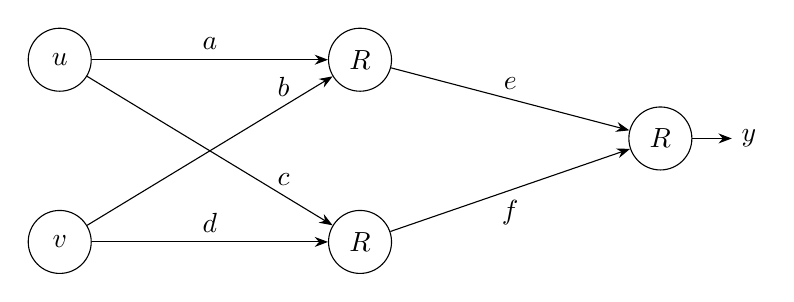
\begin{tikzpicture}[
        node distance=1.5cm and 2cm,
        neuron/.style={circle, draw, minimum size=0.8cm},
        >=Stealth
    ]
        
        \node[neuron] (u) {$u$};
        \node[neuron, below=of u] (v) {$v$};
        
        
        \node[neuron, right=of u, xshift=1cm, yshift=0cm] (h1) {$R$};
        \node[neuron, right=of v, xshift=1cm, yshift=-0cm] (h2) {$R$};
        

        \node[neuron, right=of h1, xshift=1cm, yshift=-1cm] (y_node) {$R$};
        \node[right=0.5cm of y_node] (out) {$y$};

        
        \draw[->] (u) -- node[above] {$a$} (h1);
        \draw[->] (u) -- node[pos=0.8, above] {$c$} (h2);
        \draw[->] (v) -- node[pos=0.8, above] {$b$} (h1);
        \draw[->] (v) -- node[above] {$d$} (h2);
        
        \draw[->] (h1) -- node[above] {$e$} (y_node);
        \draw[->] (h2) -- node[below] {$f$} (y_node);
        \draw[->] (y_node) -- (out);
    \end{tikzpicture}
\end{center} \\[10pt]
& Given $u = 2, v = 3,$ \\
& $a = 1, b = 1, c = 1, d = -1, e = 4, f = -1,$ \\
& which one of the following is correct? \\[10pt]
& (A) $\quad \dfrac{\partial y}{\partial a} = 8, \dfrac{\partial y}{\partial f} = 0$ \\[15pt]
& (B) $\quad \dfrac{\partial y}{\partial a} = 1, \dfrac{\partial y}{\partial f} = 0$ \\[15pt]
& (C) $\quad \dfrac{\partial y}{\partial a} = 1, \dfrac{\partial y}{\partial f} = -1$ \\[15pt]
& (D) $\quad \dfrac{\partial y}{\partial a} = 2, \dfrac{\partial y}{\partial f} = -1$ \\
\end{tabular}
\vspace{0.8cm}

\noindent
\begin{tabular}{p{1cm} p{12.5cm}}
\textbf{Q.43} & Consider game trees Tree-1 and Tree-2 as shown. The first level is a MAX agent and the second level is a MIN agent. The value in the square node is the output of the utility function. \\[10pt]
& \begin{center}
    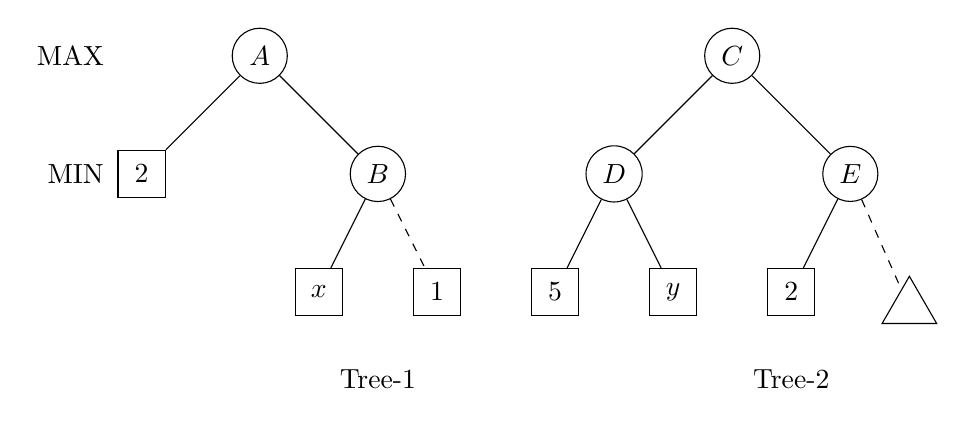
\begin{tikzpicture}[
        level distance=1.5cm,
        level 1/.style={sibling distance=3cm},
        level 2/.style={sibling distance=1.5cm},
        maxnode/.style={circle, draw, minimum size=0.7cm},
        minnode/.style={rectangle, draw, minimum size=0.6cm},
        pruned/.style={draw, dashed, -}
    ]
    
    \node (T1) at (0,0) [maxnode] {$A$}
        child {node [minnode] {2}}
        child {node [maxnode] (B) {$B$}
            child {node [minnode] {$x$}}
            child {node [minnode] {1} edge from parent[dashed]}
        };
    \node[left=1.5cm of T1] {MAX};
    \node[left=3cm of B] {MIN};
    \node[below=3.5cm of T1, xshift=1.5cm] {Tree-1};

    
    \begin{scope}[xshift=6cm]
    \node (T2) at (0,0) [maxnode] {$C$}
        child {node [maxnode] (D) {$D$}
            child {node [minnode] {5}}
            child {node [minnode] {$y$}}
        }
        child {node [maxnode] (E) {$E$}
            child {node [minnode] {2}}
            child {node [regular polygon, regular polygon sides=3, draw, minimum size=0.8cm, yshift=-0.2cm] {} edge from parent[dashed]}
        };
    \node[below=3.5cm of T2, xshift=0.75cm] {Tree-2};
    \end{scope}
    \end{tikzpicture}
\end{center} \\
& For what ranges of $x$ and $y$, the right child of node $B$ and the right child of node $E$ will be pruned by alpha-beta pruning algorithm? \\[8pt]
& (A) \quad $x \in [1, \infty)$ and $y \in (-\infty, 2]$ \\[5pt]
& (B) \quad $x \in (-\infty, 2]$ and $y \in (-\infty, 5]$ \\[5pt]
& (C) \quad $x \in (-\infty, 2]$ and $y \in [2, \infty)$ \\[5pt]
& (D) \quad $x \in [1, \infty)$ and $y \in (-\infty, 5]$ \\
\end{tabular}

\vspace{0.8cm}

\noindent
\begin{tabular}{p{1cm} p{12.5cm}}
\textbf{Q.44} & The state graph shows the action cost along the edges and the heuristic function h associated with each state. \\[10pt]
& \begin{center}
    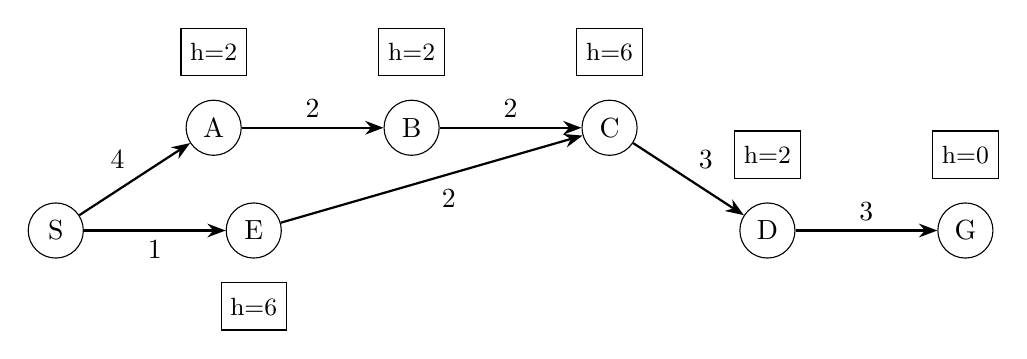
\begin{tikzpicture}[
        node distance=1.5cm and 1.8cm,
        state/.style={circle, draw, minimum size=0.7cm},
        hbox/.style={rectangle, draw, minimum size=0.6cm, font=\small},
        arrow/.style={-Stealth, thick}
    ]
        
        \node[state] (S) {S};
        \node[state, above right=0.8cm and 1.5cm of S] (A) {A};
        \node[state, right=of S] (E) {E};
        \node[state, right=of A] (B) {B};
        \node[state, right=of B] (C) {C};
        \node[state, below right=0.8cm and 1.5cm of C] (D) {D};
        \node[state, right=of D] (G) {G};


        \node[hbox, above=0.3cm of A] {h=2};
        \node[hbox, above=0.3cm of B] {h=2};
        \node[hbox, above=0.3cm of C] {h=6};
        \node[hbox, below=0.3cm of E] {h=6};
        \node[hbox, above=0.3cm of D] {h=2};
        \node[hbox, above=0.3cm of G] {h=0};

        
        \draw[arrow] (S) -- node[above left] {4} (A);
        \draw[arrow] (S) -- node[below] {1} (E);
        \draw[arrow] (A) -- node[above] {2} (B);
        \draw[arrow] (B) -- node[above] {2} (C);
        \draw[arrow] (E) -- node[below right] {2} (C);
        \draw[arrow] (C) -- node[above right] {3} (D);
        \draw[arrow] (D) -- node[above] {3} (G);
    \end{tikzpicture}
\end{center} \\
& Suppose $A^*$ algorithm is applied on this state graph using priority queue to store the frontier. In what sequence are the nodes expanded? \\[8pt]
& (A) \quad S, A, E, C, B, D, G \\[5pt]
& (B) \quad S, E, A, C, B, D, G \\[5pt]
& (C) \quad S, A, E, B, C, D, G \\[5pt]
& (D) \quad S, A, B, E, C, D, G \\
\end{tabular}

\vspace{0.8cm}

\noindent
\begin{tabular}{p{1cm} p{12.5cm}}
\textbf{Q.45} & A random experiment consists of throwing 100 fair dice, each die having six faces numbered 1 to 6. An event $A$ represents the set of all outcomes where at least one of the dice shows a 1. Then, $P(A) =$ \\[8pt]
& (A) \quad 0 \\[5pt]
& (B) \quad 1 \\[5pt]
& (C) \quad $1 - \left(\frac{5}{6}\right)^{100}$ \\[5pt]
& (D) \quad $\left(\frac{5}{6}\right)^{100}$ \\
\end{tabular}

\vspace{0.8cm}

\noindent
\begin{tabular}{p{1cm} p{12.5cm}}
\textbf{Q.46} & Consider a fact table in an OLAP application: \texttt{Facts(D1, D2, val)}, where \texttt{D1} and \texttt{D2} are its dimension attributes and \texttt{val} is a dependent attribute. Suppose attribute \texttt{D1} takes 3 values and \texttt{D2} takes 2 values, and all combinations of these values are present in the table \texttt{Facts}. How many tuples are there in the result of the following query? \\[10pt]
& \hspace{1cm} \texttt{SELECT D1, D2, sum(val)} \\
& \hspace{1cm} \texttt{FROM Facts} \\
& \hspace{1cm} \texttt{GROUP BY CUBE (D1, D2);} \\[8pt]
& (A) \quad 1 \\[5pt]
& (B) \quad 6 \\[5pt]
& (C) \quad 9 \\[5pt]
& (D) \quad 12 \\
\end{tabular}

\vspace{0.8cm}

\noindent
\begin{tabular}{p{1cm} p{12.5cm}}
\textbf{Q.47} & Consider the following Python code snippet. \\[10pt]
& \texttt{A=\{"this", "that"\}} \\
& \texttt{B=\{"that", "other"\}} \\
& \texttt{C=\{"other", "this"\}} \\[10pt]
& \texttt{while "other" in C:} \\
& \hspace{1cm} \texttt{if "this" in A:} \\
& \hspace{2cm} \texttt{A, B, C = A-B, B-C, C-A} \\[5pt]
& \hspace{1cm} \texttt{if "that" in B:} \\
& \hspace{1cm} \texttt{A, B, C = C|A, A|B, B|C} \\[10pt]
& When the above program is executed, at the end, which of the following sets contains "this"? \\[8pt]
& (A) \quad Only A \\[5pt]
& (B) \quad Only B \\[5pt]
& (C) \quad Only C \\[5pt]
& (D) \quad A, C \\
\end{tabular}

\vspace{0.8cm}

\noindent
\begin{tabular}{p{1cm} p{12.5cm}}
\textbf{Q.48} & Which of the following statements is/are correct about the rectified linear unit (ReLU) activation function defined as $\text{ReLU}(x) = \max(x, 0)$, where $x \in \mathbb{R}$? \\[8pt]
& (A) \quad ReLU is continuous everywhere \\[5pt]
& (B) \quad ReLU is differentiable everywhere \\[5pt]
& (C) \quad ReLU is not differentiable at $x = 0$ \\[5pt]
& (D) \quad $\text{ReLU}(x) = \text{ReLU}(ax)$, for all $a \in \mathbb{R}$ \\
\end{tabular}

\noindent
\begin{tabular}{p{1cm} p{12.5cm}}
\textbf{Q.49} & Consider the function $f(x) = \frac{x^3}{3} + \frac{7}{2}x^2 + 10x + \frac{133}{2}, x \in [-8, 0]$. Which of the following statements is/are correct? \\[8pt]
& (A) \quad The maximum value of $f$ is attained at $x = -5$ \\[5pt]
& (B) \quad The minimum value of $f$ is attained at $x = -2$ \\[5pt]
& (C) \quad The maximum value of $f$ is $\frac{133}{2}$ \\[5pt]
& (D) \quad The minimum value of the derivative of $f$ is attained at $x = -\frac{7}{2}$ \\
\end{tabular}

\vspace{0.6cm}

\noindent
\begin{tabular}{p{1cm} p{12.5cm}}
\textbf{Q.50} & Let $x_1, x_2, x_3, x_4, x_5$ be a system of orthonormal vectors in $\mathbb{R}^{10}$. Consider the matrix $A = x_1x_1^\top + \dots + x_5x_5^\top$. Which of the following statements is/are correct? \\[8pt]
& (A) \quad Singular values of $A$ are also its eigenvalues \\[5pt]
& (B) \quad Singular values of $A$ are either 0 or 1 \\[5pt]
& (C) \quad Determinant of $A$ is 1 \\[5pt]
& (D) \quad $A$ is invertible \\
\end{tabular}

\vspace{0.6cm}

\noindent
\begin{tabular}{p{1cm} p{12.5cm}}
\textbf{Q.51} & Let $f : \mathbb{R} \to \mathbb{R}$ be a twice-differentiable function and suppose its second derivative satisfies $f''(x) > 0$ for all $x \in \mathbb{R}$. Which of the following statements is/are ALWAYS correct? \\[8pt]
& (A) \quad $f$ has a local minima \\[5pt]
& (B) \quad There does not exist $x$ and $y, x \neq y$, such that $f'(x) = f'(y) = 0$ \\[5pt]
& (C) \quad $f$ has at most one global minimum \\[5pt]
& (D) \quad $f$ has at most one local minimum \\
\end{tabular}

\vspace{0.8cm}

\noindent
\begin{tabular}{p{1cm} p{12.5cm}}
\textbf{Q.52} & An $n \times n$ matrix $A$ with real entries satisfies the property: $\|Ax\|^2 = \|x\|^2$, for all $x \in \mathbb{R}^n$, where $\|\cdot\|$ denotes the Euclidean norm. Which of the following statements is/are ALWAYS correct? \\[8pt]
& (A) \quad $A$ must be orthogonal \\[5pt]
& (B) \quad $A = I$, where $I$ denotes the identity matrix, is the only solution \\[5pt]
& (C) \quad The eigenvalues of $A$ are either $+1$ or $-1$ \\[5pt]
& (D) \quad $A$ has full rank \\
\end{tabular}

\vspace{0.8cm}

\noindent
\begin{tabular}{p{1cm} p{12.5cm}}
\textbf{Q.53} & Consider designing a linear binary classifier $f(x) = \text{sign}(w^\top x + b), x \in \mathbb{R}^2$ on the following training data: \\[10pt]
& \text{Class-1: } $\left\{ \begin{pmatrix} 2 \\ 0 \end{pmatrix}, \begin{pmatrix} 0 \\ 2 \end{pmatrix}, \begin{pmatrix} 2 \\ 2 \end{pmatrix} \right\}$, 
  \text{Class-2: } $\left\{ \begin{pmatrix} 0 \\ 0 \end{pmatrix} \right\}$ \\[15pt]
& Hard-margin support vector machine (SVM) formulation is solved to obtain $w$ and $b$. Which of the following options is/are correct? \\[8pt]
& (A) \quad $w = \begin{pmatrix} 4 \\ 4 \end{pmatrix}$ and $b = 1$ \\[10pt]
& (B) \quad The number of support vectors is 3 \\[5pt]
& (C) \quad The margin is $\sqrt{2}$ \\[5pt]
& (D) \quad Training accuracy is $98\%$ \\
\end{tabular}

\vspace{0.8cm}

\noindent
\begin{tabular}{p{1cm} p{12.5cm}}
\textbf{Q.54} & Consider a coin-toss experiment where the probability of head showing up is $p$. In the $i^{\text{th}}$ coin toss, let $X_i = 1$ if head appears, and $X_i = 0$ if tail appears. Consider 
\[ \widehat{p} = \frac{1}{n} \sum_{i=1}^{n} X_i \]
where $n$ is the total number of independent coin tosses. Which of the following statements is/are correct? \\[8pt]
& (A) \quad $E[\widehat{p}] = p$ \\[5pt]
& (B) \quad $E[\widehat{p}] = \frac{p}{n}$ \\[5pt]
& (C) \quad As $n$ increases, variance of $\widehat{p}$ decreases \\[5pt]
& (D) \quad Variance of $\widehat{p}$ does not depend on $n$ \\
\end{tabular}

\vspace{0.8cm}

\noindent
\begin{tabular}{p{1cm} p{12.5cm}}
\textbf{Q.55} & Consider a two-class problem in $\mathbb{R}^d$ with class labels \textit{red} and \textit{green}. Let $\mu_{\text{red}}$ and $\mu_{\text{green}}$ be the means of the two classes. Given test sample $x \in \mathbb{R}^d$, a classifier calculates the squared Euclidean distance (denoted by $\|\cdot\|^2$) between $x$ and the means of the two classes and assigns the class label that the sample $x$ is closest to. That is, the classifier computes
\[ f(x) = \|\mu_{\text{red}} - x\|^2 - \|\mu_{\text{green}} - x\|^2 \]
and assigns the label \textit{red} to $x$ if $f(x) < 0$, and \textit{green} otherwise. Which of the following statements is/are correct? \\[8pt]
& (A) \quad The sample $x = 0$ is assigned the label \textit{green} if $\|\mu_{\text{red}}\| < \|\mu_{\text{green}}\|$ \\[5pt]
& (B) \quad $f$ is a linear function of $x$ \\[5pt]
& (C) \quad $f(x) = w^\top x + b$, where $w$ and $b$ are functions of $\mu_{\text{red}}$ and $\mu_{\text{green}}$ \\[5pt]
& (D) \quad $f$ is a quadratic polynomial in $x$ \\
\end{tabular}

\vspace{0.8cm}

\noindent
\begin{tabular}{p{1cm} p{12.5cm}}
\textbf{Q.56} & Consider the following two relations, named \texttt{Customer} and \texttt{Person}, in a database: \\[10pt]
& \texttt{Person (} \\
& \hspace{1.5cm} \texttt{aadhaar CHAR(12) PRIMARY KEY,} \\
& \hspace{1.5cm} \texttt{name VARCHAR(32));} \\[8pt]
& \texttt{Customer (} \\
& \hspace{1.5cm} \texttt{name VARCHAR(32),} \\
& \hspace{1.5cm} \texttt{email VARCHAR(32) PRIMARY KEY,} \\
& \hspace{1.5cm} \texttt{phone CHAR(10),} \\
& \hspace{1.5cm} \texttt{aadhaar CHAR(12),} \\[5pt]
& \hspace{1.5cm} \texttt{FOREIGN KEY (aadhaar) REFERENCES Person(aadhaar));} \\[10pt]
& Which of the following statements is/are correct? \\[8pt]
& (A) \quad \texttt{aadhaar} is a candidate key in the \texttt{Customer} relation \\[5pt]
& (B) \quad \texttt{phone} can be NULL in the \texttt{Customer} relation \\[5pt]
& (C) \quad \texttt{aadhaar} is a candidate key in the \texttt{Person} relation \\[5pt]
& (D) \quad \texttt{aadhaar} can be NULL in the \texttt{Person} relation \\
\end{tabular}

\vspace{0.8cm}
\noindent
\begin{tabular}{p{1cm} p{12.5cm}}
\textbf{Q.57} & Consider a database relation R with attributes ABCDEFG, and having the following functional dependencies: \\
& \centerline{$A \to BCEF, \quad E \to DG, \quad BC \to A$} \\[10pt]
& Which of the following statements is/are correct? \\[8pt]
& (A) \quad A is the only candidate key of R \\[5pt]
& (B) \quad A, BC are the candidate keys of R \\[5pt]
& (C) \quad A, BC, E are the candidate keys of R \\[5pt]
& (D) \quad Relation R is not in Boyce-Codd Normal Form (BCNF) \\
\end{tabular}

\vspace{0.8cm}
\noindent
\begin{tabular}{p{1cm} p{12.5cm}}
\textbf{Q.58} & Let $G$ be a simple, unweighted, and undirected graph. A subset of the vertices and edges of $G$ are shown below. \\[10pt]
& \begin{center}
    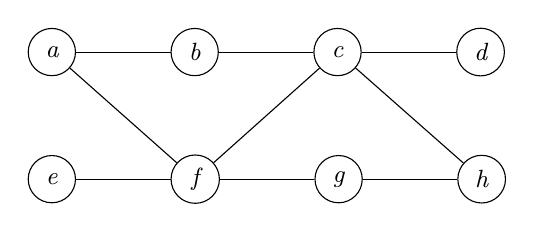
\begin{tikzpicture}[
    node distance=1cm and 1.2cm,
    vertex/.style={circle, draw, minimum size=0.6cm, font=\small\itshape}
]
    
    \node[vertex] (a) {a};
    \node[vertex, right=of a] (b) {b};
    \node[vertex, right=of b] (c) {c};
    \node[vertex, right=of c] (d) {d};
    \node[vertex, below=of a] (e) {e};
    \node[vertex, right=of e] (f) {f};
    \node[vertex, right=of f] (g) {g};
    \node[vertex, right=of g] (h) {h};

    
    \draw (a) -- (b); \draw (b) -- (c); \draw (c) -- (d);
    \draw (e) -- (f); \draw (f) -- (g); \draw (g) -- (h);
    \draw (a) -- (f); \draw (f) -- (c); \draw (c) -- (h);
\end{tikzpicture}
\end{center} \\
& It is given that $a-b-c-d$ is a shortest path between $a$ and $d$; $e-f-g-h$ is a shortest path between $e$ and $h$; $a-f-c-h$ is a shortest path between $a$ and $h$. Which of the following is/are NOT the edges of $G$? \\[8pt]
& (A) \quad $(b, d)$ \quad (B) \quad $(b, g)$ \quad (C) \quad $(b, h)$ \quad (D) \quad $(e, g)$ \\
\end{tabular}

\vspace{0.8cm}

\noindent
\begin{tabular}{p{1cm} p{12.5cm}}
\textbf{Q.59} & Let $f : \mathbb{R} \to \mathbb{R}$ be such that $|f(x) - f(y)| \leq (x - y)^2$ for all $x, y \in \mathbb{R}$. Then $f(1) - f(0) = \rule{2cm}{0.4pt}$ (Answer in integer) \\
\end{tabular}

\vspace{0.8cm}

\noindent
\begin{tabular}{p{1cm} p{12.5cm}}
\textbf{Q.60} & Let $D = \{x^{(1)}, \dots, x^{(n)}\}$ be a dataset of $n$ observations where each $x^{(i)} \in \mathbb{R}^{100}$. It is given that $\sum_{i=1}^{n} x^{(i)} = 0$. The covariance matrix computed from $D$ has eigenvalues $\lambda_i = 100^{2-i}, 1 \leq i \leq 100$. Let $u \in \mathbb{R}^{100}$ be the direction of maximum variance with $u^\top u = 1$. \\[10pt]
& The value of 
\[ \frac{1}{n} \sum_{i=1}^{n} (u^\top x^{(i)})^2 =\rule{2cm}{0.4pt} \]

\end{tabular}

\vspace{0.8cm}

\noindent
\begin{tabular}{p{1cm} p{12.5cm}}
\textbf{Q.61} & A bag contains $5$ white balls and $10$ black balls. In a random experiment, $n$ balls are drawn from the bag one at a time with replacement. Let $S_n$ denote the total number of black balls drawn in the experiment. \\[10pt]
& The expectation of $S_{100}$ denoted by $E[S_{100}] = \rule{2cm}{0.4pt} $ \\
& (Round off to one decimal place) \\
\end{tabular}

\vspace{0.8cm}
\noindent
\begin{tabular}{p{1cm} p{12.5cm}}
\textbf{Q.62} & Consider the following tables, \textbf{Loan} and \textbf{Borrower}, of a bank. \\[10pt]
&\begin{center}
   
    \begin{minipage}[t]{0.2 \textwidth}
        \centering
        \begin{tabular}{|c|c|c|}
            \hline
            \multicolumn{3}{|c|}{\textbf{Loan}} \\ \hline
            \textbf{loan\_num} & \textbf{branch\_name} & \textbf{amount} \\ \hline
            L11 & Banjara Hills & 90000 \\ \hline
            L14 & Kondapur & 50000 \\ \hline
            L15 & SR Nagar & 40000 \\ \hline
            L22 & SR Nagar & 25000 \\ \hline
            L23 & Balanagar & 80000 \\ \hline
            L25 & Kondapur & 70000 \\ \hline
            L19 & SR Nagar & 65000 \\ \hline
        \end{tabular}
    \end{minipage}
    \hfill 
    \begin{minipage}[t]{0.2\textwidth}
        \centering
        \begin{tabular}{|c|c|}
            \hline
            \multicolumn{2}{|c|}{\textbf{Borrower}} \\ \hline
            \textbf{customer\_name} & \textbf{loan\_num} \\ \hline
            Anand & L11 \\ \hline
            Karteek & L11 \\ \hline
            Karteek & L14 \\ \hline
            Ankita & L15 \\ \hline
            Gopal & L19 \\ \hline
            Karteek & L22 \\ \hline
            Karteek & L23 \\ \hline
            Sunil & L23 \\ \hline
            Sunil & L25 \\ \hline
        \end{tabular}
    \end{minipage}
\end{center}\\[10pt]

\vspace{0.5cm}
        
& Query: $\pi_{\text{branch\_name, customer\_name}}(\text{Loan} \bowtie \text{Borrower}) \div \pi_{\text{branch\_name}}(\text{Loan})$ \\
& where $\bowtie$ denotes natural join. \\[10pt]
& The number of tuples returned by the above relational algebra query is \underline{\hspace{2cm}} \\
& (Answer in integer) \\
\end{tabular}

\vspace{0.8cm}

\noindent
\begin{tabular}{p{1cm} p{12.5cm}}
\textbf{Q.63} & Consider the following Python code snippet. \\
& \begin{minipage}{10cm}
\begin{verbatim}
def f(a, b):
    if (a == 0):
        return b
    if (a % 2 == 1):
        return 2 * f((a - 1) / 2, b)
    return b + f(a - 1, b)

print(f(15, 10))
\end{verbatim}
\end{minipage} \\[10pt]
& The value printed by the code snippet is \underline
{\hspace{1cm}}. \\
& (Answer in integer) \\
\end{tabular}

\vspace{0.8cm}

\noindent
\begin{tabular}{p{1cm} p{12.5cm}}
\textbf{Q.64} & Consider the following pseudocode. \\
& \begin{minipage}{10cm}
\begin{verbatim}
Create empty stack S
Set x=0, flag=0, sum=0
Push x onto S
while (S is not empty){
    if (flag equals 0){
        Set x = x+1
        Push x onto S}
    if (x equals 8):
        Set flag=1
    if (flag equals 1){
        x = Pop(S)
        if (x is odd):
            Pop(S)
        Set sum = sum + x}
}
Output sum
\end{verbatim}
\end{minipage} \\[10pt]
& The value of \texttt{sum} output by a program executing the above pseudocode is \underline{\hspace{1.5cm}}. \\
& (Answer in integer) \\
\end{tabular}

\vspace{0.8cm}

\noindent
\begin{tabular}{p{1cm} p{12.5cm}}
\textbf{Q.65} & Consider a directed graph $G = (V, E)$, where $V = \{0, 1, 2, \dots, 100\}$ and $E = \{(i, j) : 0 < j - i \leq 2, \text{ for all } i, j \in V\}$. Suppose the adjacency list of each vertex is in \textit{decreasing} order of vertex number, and depth-first search (DFS) is performed at vertex 0. The number of vertices that will be discovered after vertex 50 is \underline{\hspace{1.5cm}}. \\
& (Answer in integer) \\
\end{tabular}


\end{document}
